\documentclass[12pt]{article}
\usepackage{url, graphicx}

% page layout
\setlength{\topmargin}{-0.25in}
\setlength{\textheight}{9.5in}
\setlength{\headheight}{0in}
\setlength{\headsep}{0in}

% problem formatting
\newcommand{\problemname}{Problem}
\newcounter{problem}

% math
\newcommand{\dd}{\mathrm{d}}

% primary units
\newcommand{\rad}{\mathrm{rad}}
\newcommand{\kg}{\mathrm{kg}}
\newcommand{\m}{\mathrm{m}}
\newcommand{\s}{\mathrm{s}}

% secondary units
\renewcommand{\deg}{\mathrm{deg}}
\newcommand{\km}{\mathrm{km}}
\newcommand{\mi}{\mathrm{mi}}
\newcommand{\h}{\mathrm{h}}
\newcommand{\ns}{\mathrm{ns}}
\newcommand{\J}{\mathrm{J}}
\newcommand{\eV}{\mathrm{eV}}
\newcommand{\W}{\mathrm{W}}

% derived units
\newcommand{\mps}{\m\,\s^{-1}}
\newcommand{\mph}{\mi\,\h^{-1}}
\newcommand{\mpss}{\m\,\s^{-2}}

% random stuff
\sloppy\sloppypar\raggedbottom\frenchspacing\thispagestyle{empty}

\begin{document}

\noindent
Name: \rule[-1ex]{0.55\textwidth}{0.1pt}
NetID: \rule[-1ex]{0.2\textwidth}{0.1pt}

\section*{NYU Physics I---Term Exam 3}

\paragraph{\problemname~\theproblem:}\refstepcounter{problem}%
(from lecture 2018-10-16)
Remember this free-body diagram for the light table? We obtained an expression
for the net torque on the table when we put the reference point at the location
at which the force $N_B$ acts.
What would we have obtained for the net torque if we had put the reference point
at the location at which the force $N_A$ acts?
Keep the same sign convention (counter-clockwise is positive torque).\\
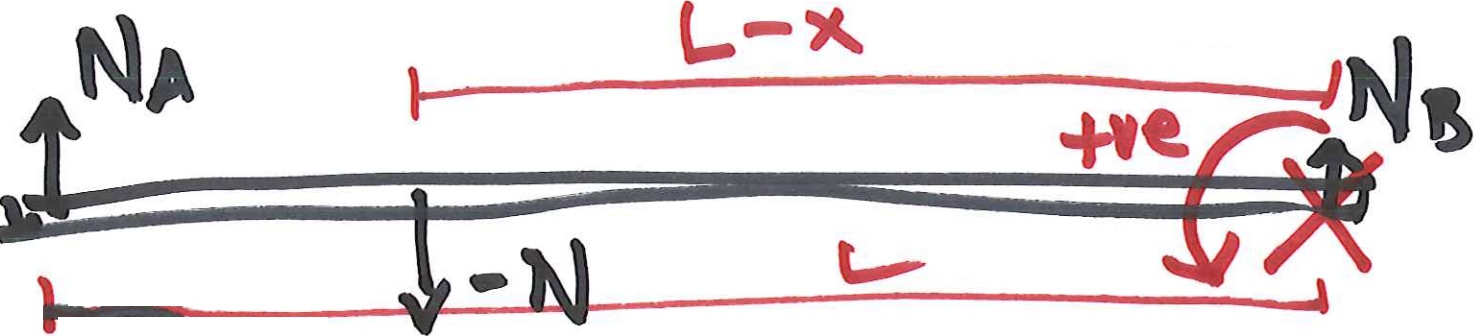
\includegraphics[width=3in]{../jpg/light_table.jpg}

\vfill

\paragraph{\problemname~\theproblem:}\refstepcounter{problem}%
(from lecture 2018-10-18)
Without using a calculator, estimate the sine of the angle $1.2~\deg$.
Use the small-angle approximation! (\emph{Hint:} Degrees aren't radians.)

\vfill

\paragraph{\problemname~\theproblem:}\refstepcounter{problem}%
(from bouncing worksheet)
An elastic ball of mass $m$ heads at speed $v$ towards a huge wall.
Its initial velocity is at an angle of $\theta$ to the normal.
Imagine that the collision is perfectly elastic and the
wall is perfectly frictionless, so the ``angle of incidence equals the
angle of reflection''. What is the magnitude of the momentum change of the ball (final
minus initial)?
Give your answer in terms of the symbols in the diagram.
\marginpar{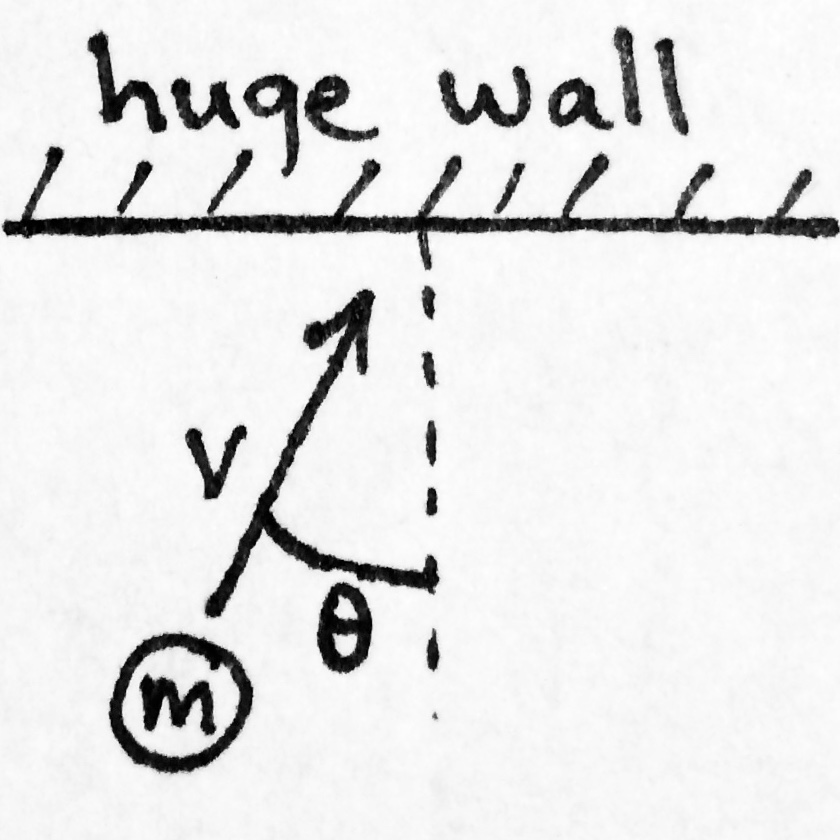
\includegraphics[width=1in]{../jpg/ballwall.jpg}}

\vfill
~
\clearpage
\paragraph{\problemname~\theproblem:}\refstepcounter{problem}%
(from oscillations worksheet)
The $x$-axis position $x$ of a particle as a function of time is
$$
x(t) = A\,\cos(\omega t) \quad .
$$
What is the maximum $x$-direction velocity $v_{\mathrm{max}}$ that the
particle obtains in this motion, and what is the period $T$ of the
velocity oscillation?  Give your answers in terms of $A$ and $\omega$.

\vfill

\paragraph{\problemname~\theproblem:}\refstepcounter{problem}%
(from Problem Set 5)
A student of mass $m_\mathrm{student}=80\,\kg$ stands at rest next to
a block of ice of mass $m_\mathrm{ice}=320\,\kg$, also at rest, on a
frictionless frozen lake.  The student pushes on the block. After the
push is completed, the block is moving in the positive $x$ direction at $1\,\mps$
relative to the frozen lake.
What is the student's velocity (relative to the lake) after the push?


\vfill

\paragraph{\problemname~\theproblem:}\refstepcounter{problem}%
(from Problem Set 6)
If a block of mass $M$ is dragged a distance $h$ across a horizontal floor,
how much heat $Q$ is generated? Assume that the acceleration due to
gravity is $g$, that the friction is kinetic with
coefficient $\mu$, and that the force pulling the block is purely
horizontal.

\vfill
~
\end{document}
